\documentclass{article} % For LaTeX2e
\usepackage{nips15submit_e,times}
\usepackage{hyperref}
\usepackage{url}
\usepackage{graphicx}
\usepackage{float}
\usepackage{amsmath}
%\usepackage{listings}
%\documentstyle[nips14submit_09,times,art10]{article} % For LaTeX 2.09


\title{Weekly Report(Apr 9,2018-Apr 15, 2018)}

\author{
Liu Junnan\\
\texttt{ljnsjtu@hotmail.com}
}
% The \author macro works with any number of authors. There are two commands
% used to separate the names and addresses of multiple authors: \And and \AND.
%
% Using \And between authors leaves it to \LaTeX{} to determine where to break
% the lines. Using \AND forces a linebreak at that point. So, if \LaTeX{}
% puts 3 of 4 authors names on the first line, and the last on the second
% line, try using \AND instead of \And before the third author name.

\newcommand{\fix}{\marginpar{FIX}}
\newcommand{\new}{\marginpar{NEW}}

%\nipsfinalcopy % Uncomment for camera-ready version

\begin{document}


\maketitle

\begin{abstract}
    This week I dealt with hardware and software problems of my computer in lab, and learned ``How to Use Git and GitHub" and machine learning course.
\end{abstract}

\section{Work done}
This is the first week that I joined AISIG, during which I have done quite different tasks since everything is new here and I have to get used to it. Mainly what I did this week are:
\begin{itemize}
    \item Reinstalling operation system and set up coding environment
    \item Learning the course ``how to use Git and GitHub" to deal with the problem of version control and collaboration of other coders
    \item Learning machine learning on Coursera held by Andrew Ng
\end{itemize}
Since I'm familiar with theory courses like linear algebra, possibility and statistics, and programming languages like C/C++ and Python, I just skip them and continue to the rest.

\subsection{Reinstalling OS}
The computer in the lab I use has dual-OS(Win 10 and Ubuntu 14.04) with bootloader grub2. However, Ubuntu failed to boot and information displayed on the screen was quite confusing. Since Dr. Song Tao said it was okey to format the whole disk, I decided to format the partitions used by Ubuntu and to re-partition the disk to fit my need. Besides, I added an SSD to the computer to make it work faster.

Then a tricky problem occurred that after formatting the disk that contained Ubuntu and shutting down the computer, it failed to boot Win 10. I soon realized that the bootloader--grub2 was installed on Ubuntu rather than Win 10, and while I formatted Ubuntu, grub2 was also erased, which led to the failure.

After I figured out what caused the failure, the solution was not difficult. I downloaded a Win10 PE on Internet on my laptop and created a bootable U disk. Then I used a boot-repair tool provided by the Win PE and set EasyBSD as the bootloader. After that, the computer succeeded to boot.

What I learn from the whole process is that one should always check the status and, probably more importantly, the location of the bootloader before he tries to format any of his operating system.

\subsection{Learning Git and GitHub}
Although I have used GitHub for years, it just works as a search engine and a cloud for me since I just search the code I want on it and backup my code on it. Following the course \href{https://www.udacity.com/course/how-to-use-git-and-github--ud775}{How to use Git and GitHub}, I learned plenty useful commands and techniques to
\begin{enumerate}
    \item do version control
    \item collaborate with other programmers.
\end{enumerate}

For the first part, a common issue is that one wants to add some new features to the project, but he also wants the original code to still work fine and correctly. A solution without version control is that you can copy and paste the original project, rename it as, say, "modified\_project", and work on the new one. But Git gives a new solution to it that you can type "git branch new\_features \& git checkout new\_feature" to create a new branch named "new\_feature", so that you can do anything you want on it and the original one will still remain unchanged.

For the second, open source projects become popular these years, and a open source project, especially a big one, requires more than a single developer to implement and upgrade the code. GitHub provides a practical solution that a core team maintains the core functions of the project called master branch, while contributors pull the master branch to their own computers and create their own branches that modify the master branch. When a new feature is done and debugged, a contributor then creates a "pull-request" on the project's webpage on GitHub, which requests the core developers to pull their branch and merge the new feature to the master branch. Once the pull request is agreed, other developers can synchronize their master branch and find the new feature.

Git and GitHub really provides powerful tools in terms of version control and collaboration with others, but there are much more commands that are not mentioned or detailed in the videos. I believe if I apply Git to everyday coding, I will get to know how to use it well.
% I believe if you apply Git to everyday coding, problems will occur and be addressed, and after that you

%\begin{listings}
%git branch new_features & git checkout new_feature
%\end{listings}

\subsection{Machine Learning Course}
I enrolled in the \href{https://www.coursera.org/learn/machine-learning}{course} on Coursera. Actually I learned a bit of machine learning during undergraduate. But it has been a while since I didn't use it, so I had to refresh my knowledge to continue the rest of the training.

\subsubsection{Linear Regression}
The task of linear regression is quite straightforward:

Given $m$ examples of $(x,y)$, where $x$'s are input variables/features, and $y$'s are output variables/``target" value, find the line that fits the examples best.

To address the problem, linear regression first defines the hypothesis
$$h_\theta(x)=\theta_0+\theta_1 x$$
Then the original task is equivalent to choosing the proper $\theta_1,\theta_2$ so that $h_\theta(x)$ is close to $y$ for training example $(x,y)$.

To solve this, define
$$J(\theta_0, \theta_1)=\frac{1}{2m}\sum_{i=1}^m (h_\theta(x^{(i)}) - y^{(i)})^2$$
where $x^{(i)}$ and $y^{(i)}$ represent the input and output values of the $i$th example respectively.

 The task turns out to minimize the value of cost function $J(\theta_0,\theta_1)$, written in math language, $$\arg\min_{\theta_0,\theta_1} J(\theta_0,\theta_1)$$

Then it comes gradient descent, a fundamental and still powerful optimization algorithm. The intuition of gradient descent is that when one wants to go down a hill in a fastest manner, he should make every step towards the the steepest direction downward(Shown in Fig. \ref{fig:gd}). So it is also called steepest descent algorithm.

\begin{figure}[H]
\centering
%\framebox[4.0in]{$\;$}
%\fbox{\rule[-.5cm]{0cm}{4cm} \rule[-.5cm]{4cm}{0cm}}
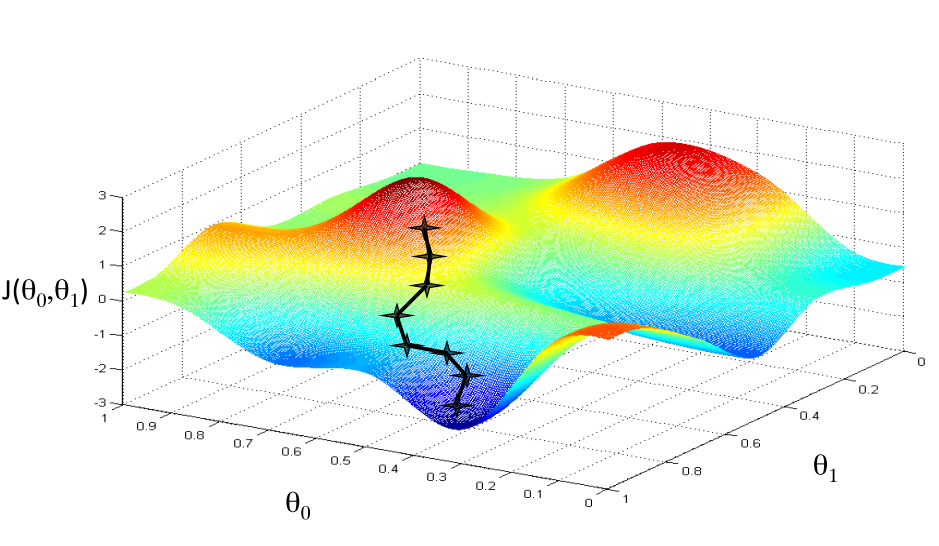
\includegraphics[width=0.5\textwidth]{gd.png}
\caption{Gradient Descent.}
\label{fig:gd}
\end{figure}

Concretely, gradient descent is given as

repeat until convergence

\begin{eqnarray*}
    \theta_0 &:=& \theta_0 - \alpha \frac{\partial}{\partial \theta_0}J(\theta_1, \theta_2) \\
        &=& \theta_0 - \alpha \frac{1}{m} \sum_{i=1}^m (h_\theta(x^{(i)})-y^{(i)})\\
    \theta_1 &:=& \theta_1 - \alpha \frac{\partial}{\partial \theta_1}J(\theta_1, \theta_2) \\
        &=& \theta_1 - \alpha \frac{1}{m} \sum_{i=1}^m (h_\theta(x^{(i)})-y^{(i)})x^{(i)}
\end{eqnarray*}

where $\alpha$ is a parameter called learning rate.

With gradient descent, we can easily minimize cost function $J(\theta_1,\theta_2)$ and fit the training data.

\subsubsection{Logistic Regression}
Classification is a classic problem in machine learning. Instead of using linear regression, which is most likely to produce bad results, we apply logistic regression to solving it.

The simplified version of classification is that,

Given $m$ examples of $(x,y)$, where $y \in \{0,1\}$, find a curve that separates positives examples from negative ones.

To solve this problem, logistic regression first defines the hypothesis as
\begin{eqnarray*}
    h_\theta(x)&=&g(\theta^T x)\\
    g(z)&=&\frac{1}{1+e^{-\theta^T x}}
\end{eqnarray*}

and cost function as
\begin{eqnarray}
    J(\theta)=-y \log(h_\theta(x)) - (1 - y)(1 - \log(h_\theta(x)))
    \label{eq:cost function}
\end{eqnarray}

%\begin{eqnarray*}
%J(\theta) &=& \frac{1}{m}\sum_{i=1}^m Cost(h_\theta(x^{(i)}),y^{(i)})\\
%Cost(h_\theta(x), y) &=&
%\left \{
%    \begin{array}{ll}
%        -\log(h_\theta(x)) & \mbox{if }y=1\\
%        -\log(1-h_\theta(x)) & \mbox{if }y=0
%    \end{array}
%\right.
%\end{eqnarray*}

%Actually $Cost(h_\theta(x),y)$ can be written in one line:
%$$Cost(h_\theta(x),y)=-y \log(h_\theta(x)) - (1 - y)(1 - \log(h_\theta(x)))$$

Like linear regression, we also need to compute the partial derivative with respect to $\theta_i$ in cost function $J(\theta)$.
However, the partial derivative is more difficult to compute compared to linear regression. The following is how I compute the partial derivatives.

Define
$$ \alpha^{(i)}=y^{(i)}\log (h_\theta(x^{(i)})) $$
and
$$ \beta^{(i)}=(1-y^{(i)})\log (1-h_\theta(x^{(i)})) $$

So equation\ref{eq:cost function} can be simplified as $$J(\theta)=\frac{1}{m} \sum_{i=1}^{m} (- \alpha^{(i)} - \beta^{(i)})$$

To derive the partial derivative w.r.t. $\theta_j$, we can first compute $\frac{\partial h_\theta(x^{(i)})}{\partial \theta_j}$ because it is used both in $\alpha$ and $\beta$
\begin{eqnarray*}
    \frac{\partial h_\theta(x^{(i)})}{\partial \theta_j} &=& \frac{\partial}{\partial \theta_j} (1+\exp(-(\theta_0+\theta_1 x^{(i)}_1+\theta_2 x^{(i)}_2...+\theta_n x^{(i)}_n))^{-1})\\
    &=& (1 + \exp(-\theta^T x))^{-2} \cdot \exp(-\theta^T x) \cdot x^{(i)}_j\\
%    &=& (1 + \frac{1}{\exp(-\theta^T x)}^{2}) \cdot \exp(-\theta^T x) \cdot x^{(i)}_j\\
    &=& h_\theta(x)^2 \cdot \exp(-\theta^T x) \cdot x^{(i)}_j
\end{eqnarray*}

then compute the term $\alpha^{(i)}$
\begin{eqnarray*}
    \frac{\partial \alpha^{(i)}}{\partial \theta_j} &=& y^{(i)} \cdot \frac{\partial}{\partial \theta_j} \log (h_\theta(x^{(i)}))\\
    &=& y^{(i)} \cdot \frac{1}{h_{\theta}(x)} \cdot \frac{\partial h_\theta(x)}{\partial \theta_j}\\
%    &=&  y^{(i)} \cdot \frac{1}{h_{\theta}(x)} \cdot h_\theta(x)^2 \cdot \exp(-\theta^T X) \cdot x^{(i)}\\
%    &=& y^{(i)} \cdot \frac{1}{h_{\theta}(x)} \cdot exp(-\theta^T X) \cdot x^{(i)}
\end{eqnarray*}

and similarly $\beta^{(i)}$
\begin{eqnarray*}
    \beta^{(i)} &=& (1-y^{(i)}) \cdot \log (1-h_\theta(x^{(i)}))\\
    &=& (1-y^{(i)}) \cdot \frac{1}{1-h_\theta(x^{(i)})} \cdot \frac{\partial}{\partial \theta_j} (1-h_\theta(x^{(i)}))\\
    &=& -(1-y^{(i)}) \cdot \frac{1}{1-h_\theta(x^{(i)})} \cdot \frac{\partial h_\theta(x^{(i)})}{\partial \theta_j}
\end{eqnarray*}

and now we can put them together as follows
\begin{eqnarray}
\begin{split}
    - \alpha^{(i)} - \beta^{(i)} &= \left[ - y^{(i)} \cdot \frac{1}{h_{\theta}(x)} \cdot \frac{\partial h_\theta(x)}{\partial \theta_j} \right] - \left[ -(1-y^{(i)}) \cdot \frac{1}{1-h_\theta(x^{(i)})} \cdot \frac{\partial h_\theta(x^{(i)})}{\partial \theta_j} \right]\\
     &= \left[ \frac{1-y^{(i)}}{1-h_\theta(x^{(i)})} - \frac{y^{(i)}}{h_\theta(x^{(i)})} \right] \cdot \frac{\partial h_\theta(x^{(i)})}{\partial \theta_j}
\end{split}
     \label{eq:lr gd}
\end{eqnarray}

Here is the most tricky part of the whole derivation. At the first glance at the first term of equation\ref{eq:lr gd}, I believe there is no way to be more simplified. But it turns out that I am wrong.
\begin{eqnarray*}
    \left[ \frac{1-y^{(i)}}{1-h_\theta} - \frac{y^{(i)}}{h_\theta} \right] \cdot \frac{\partial h_\theta(x^{(i)})}{\partial \theta_j} &=& \frac{h_\theta - y^{(i)}}{(1- h_\theta)) h_\theta} \cdot \left[ h^2_\theta \cdot \exp(-\theta^T x) \cdot x^{(i)} \right]\\
    &=& (h_\theta(x^{(i)})-y^{(i)})x^{(i)} \cdot \frac{h_\theta(x^{(i)})}{1-h_\theta(x^{(i)})} \exp(-\theta^T x)\\
    &=& (h_\theta(x^{(i)})-y^{(i)})x^{(i)} \cdot \frac{\frac{1}{1+\exp(-\theta^T x)}}{1-\frac{1}{1+\exp(-\theta^T x)}} \exp(-\theta^T x)\\
    &=& (h_\theta(x^{(i)})-y^{(i)})x^{(i)} \cdot \frac{1}{\exp(-\theta^T x)}\exp(-\theta^T x)\\
    &=& (h_\theta(x^{(i)})-y^{(i)})x^{(i)}
\end{eqnarray*}

Therefore
\begin{eqnarray}
    \frac{\partial J(\theta)}{\partial \theta_j}&=& \frac{1}{m}\sum_{i=1}^m ( -\alpha^{(i)} - \beta^{(i)} )\\
    &=& \frac{1}{m}\sum_{i=1}^m (h_\theta(x^{(i)})-y^{(i)})x^{(i)}_j
\end{eqnarray}


\subsubsection{Neural Network}
Logistic regression works pretty well on linear separable problems. But in the real world, there are much more linear non-separable problems that logistic regression can't solve. Neural network provides a general method to solve classification problems. A neural network is a layered structure, each layer of which are several computing units that take the output of previous layer that link to it as input and perform activation function on the sum of them and then produce the output. The series of procedures of computing the output of the last layer is called forward propagation, which represents the prediction of the input fed to the neural network. The algorithm used to optimize the parameters is back propagation algorithm, which is an application of chain rules of calculus. Back propagation is kind of expansion of gradient descent that performs on multi-layered structure. With a lot iterations of forward propagation and back propagation, the model is most likely to be a well-fitted.

\section{Plans}
In the next week I will continue to learn the machine learning course.

\end{document}
